
\Problem{Cercles fractals}

\Statement

Voleu pintar en Python fractals tant xulos com aquest?

\begin{center}
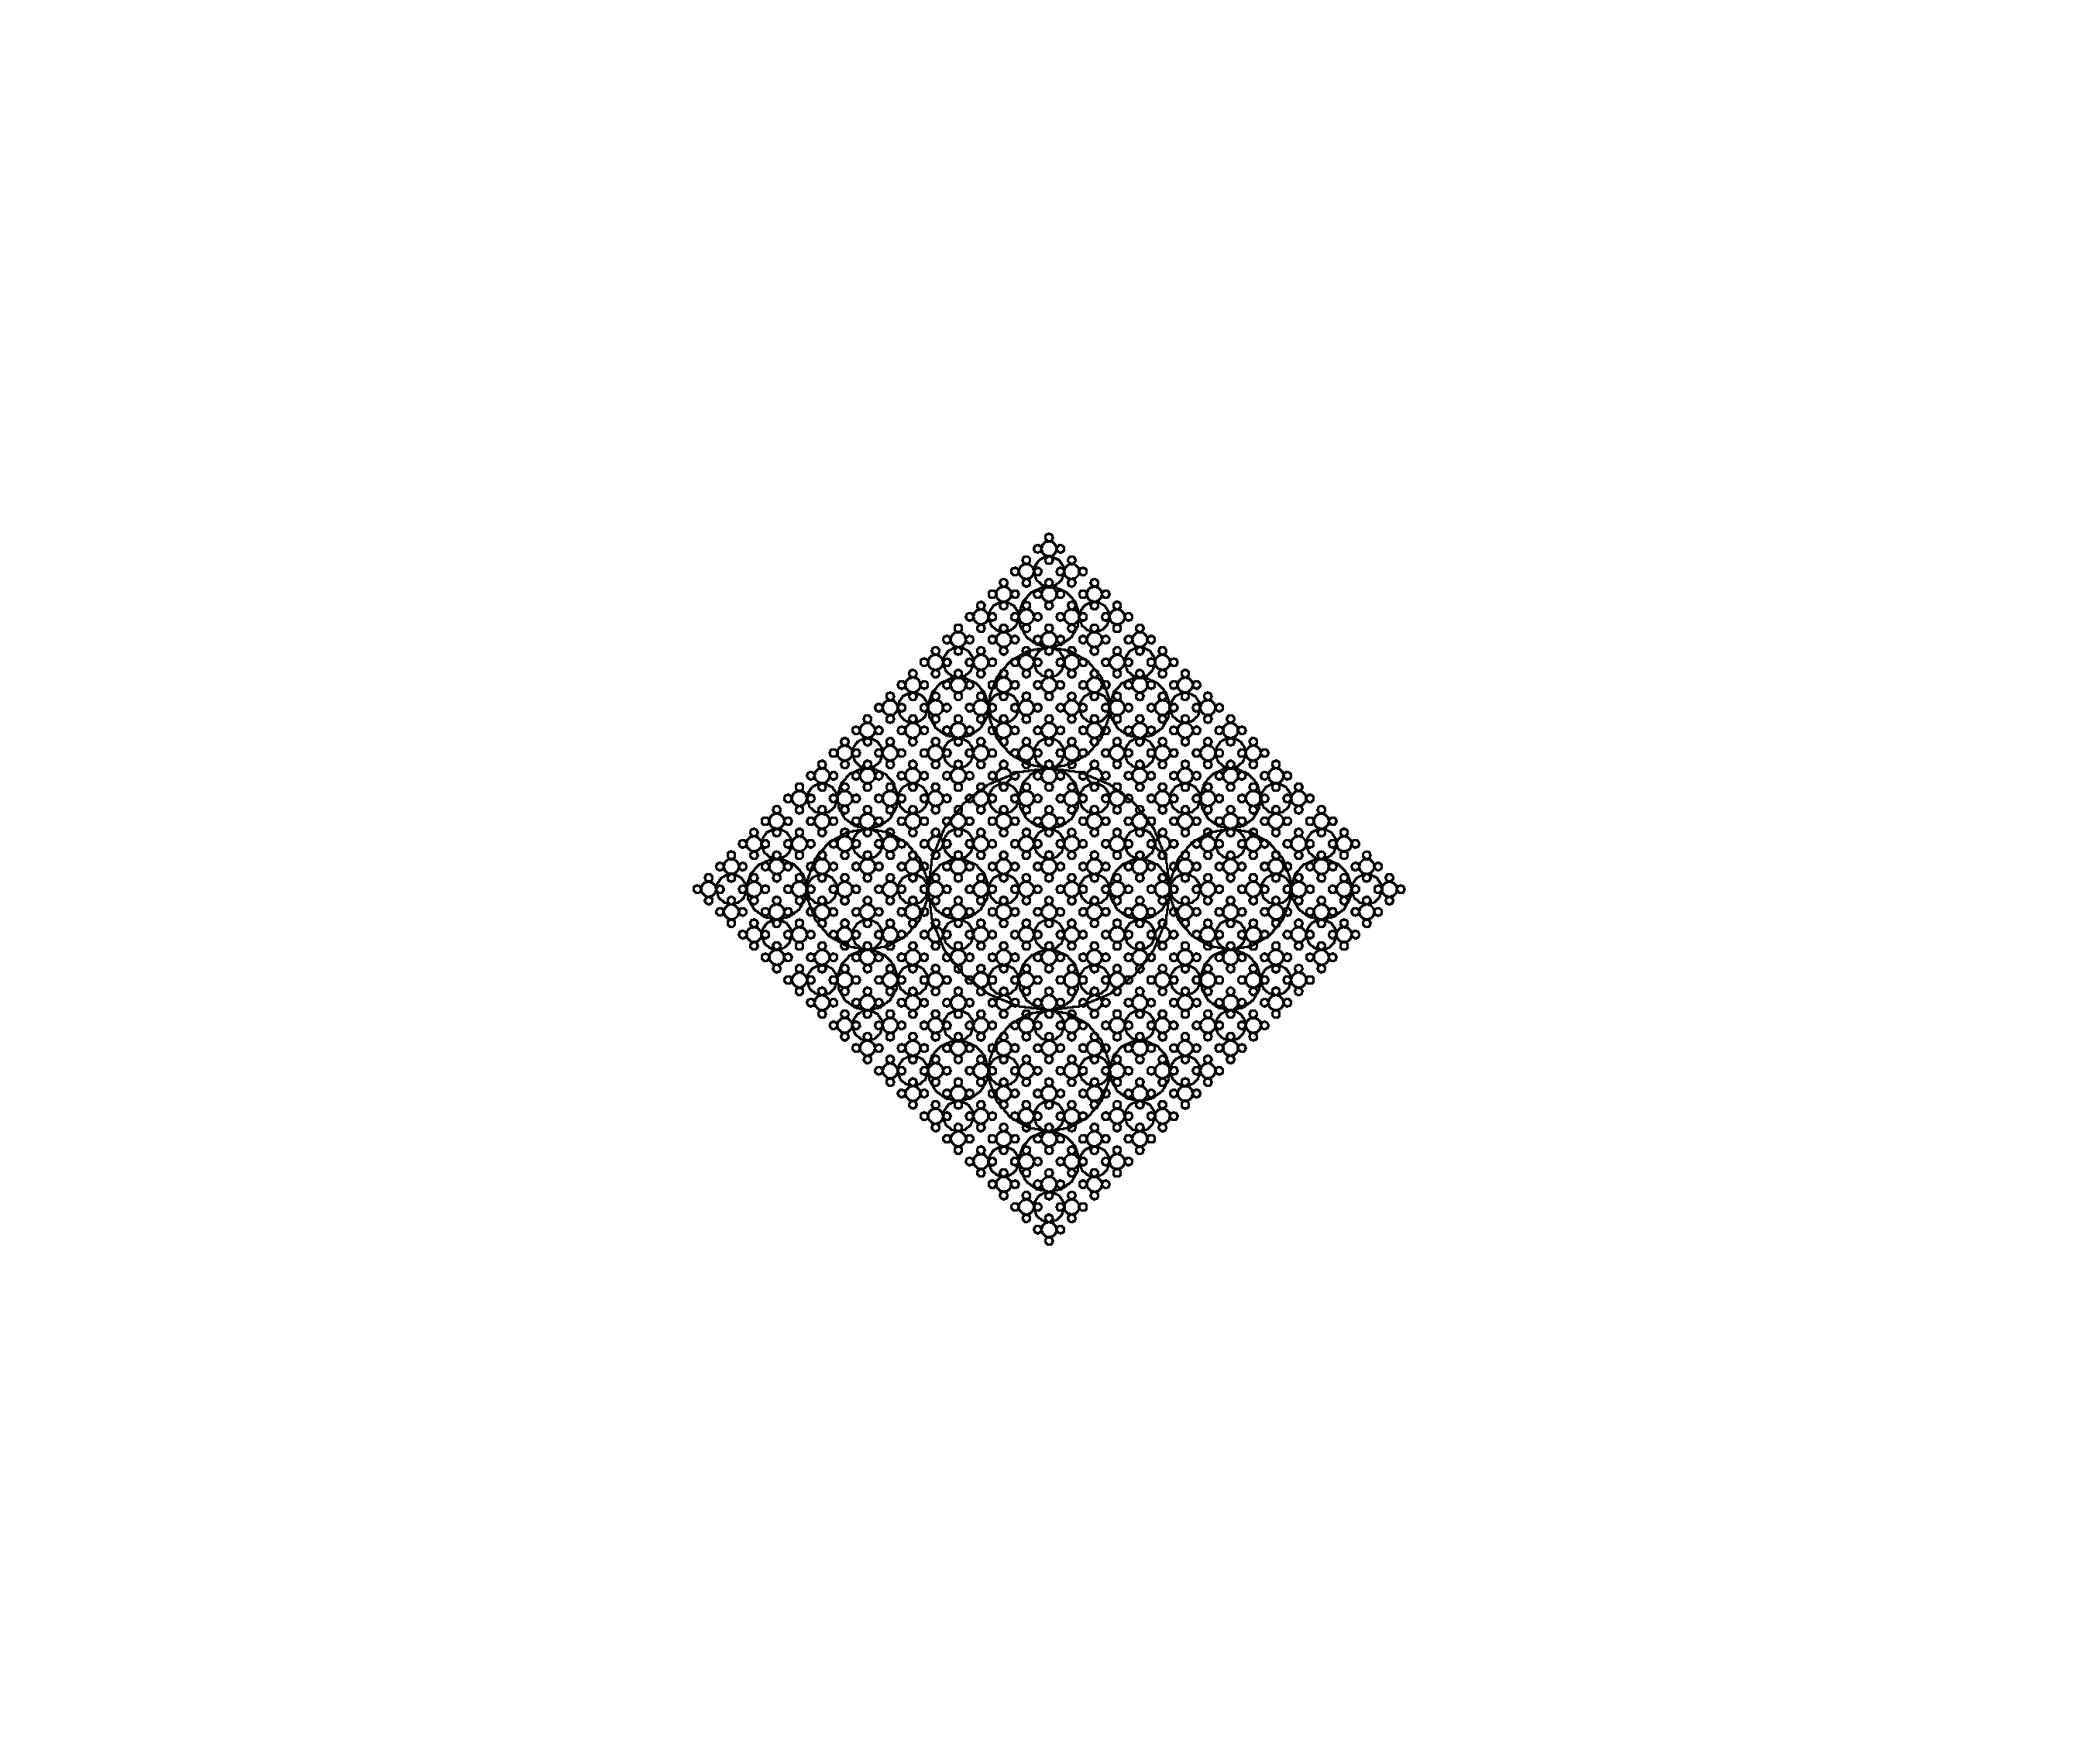
\includegraphics[trim=450 300 450 325,height=10cm]{6.eps}
\end{center}

Per pintar un fractal de $n\ge1$ nivells de mida $d$, cal pintar un cercle
de mida $d$, i quatre fractals al seu damunt, avall, esquerra i dreta
amb $n-1$ nivells i mida $d/2$. Un fractal de zero nivells és buit.

\bigskip

Per exemple, aquests són els fractals amb 1, 2, 3, 4, 5 i 6 nivells:

\begin{center}
1 ~
\fbox{

\includegraphics[trim=450 300 450 325,height=3.5cm]{1.eps}
}
\qquad
2 ~
\fbox{
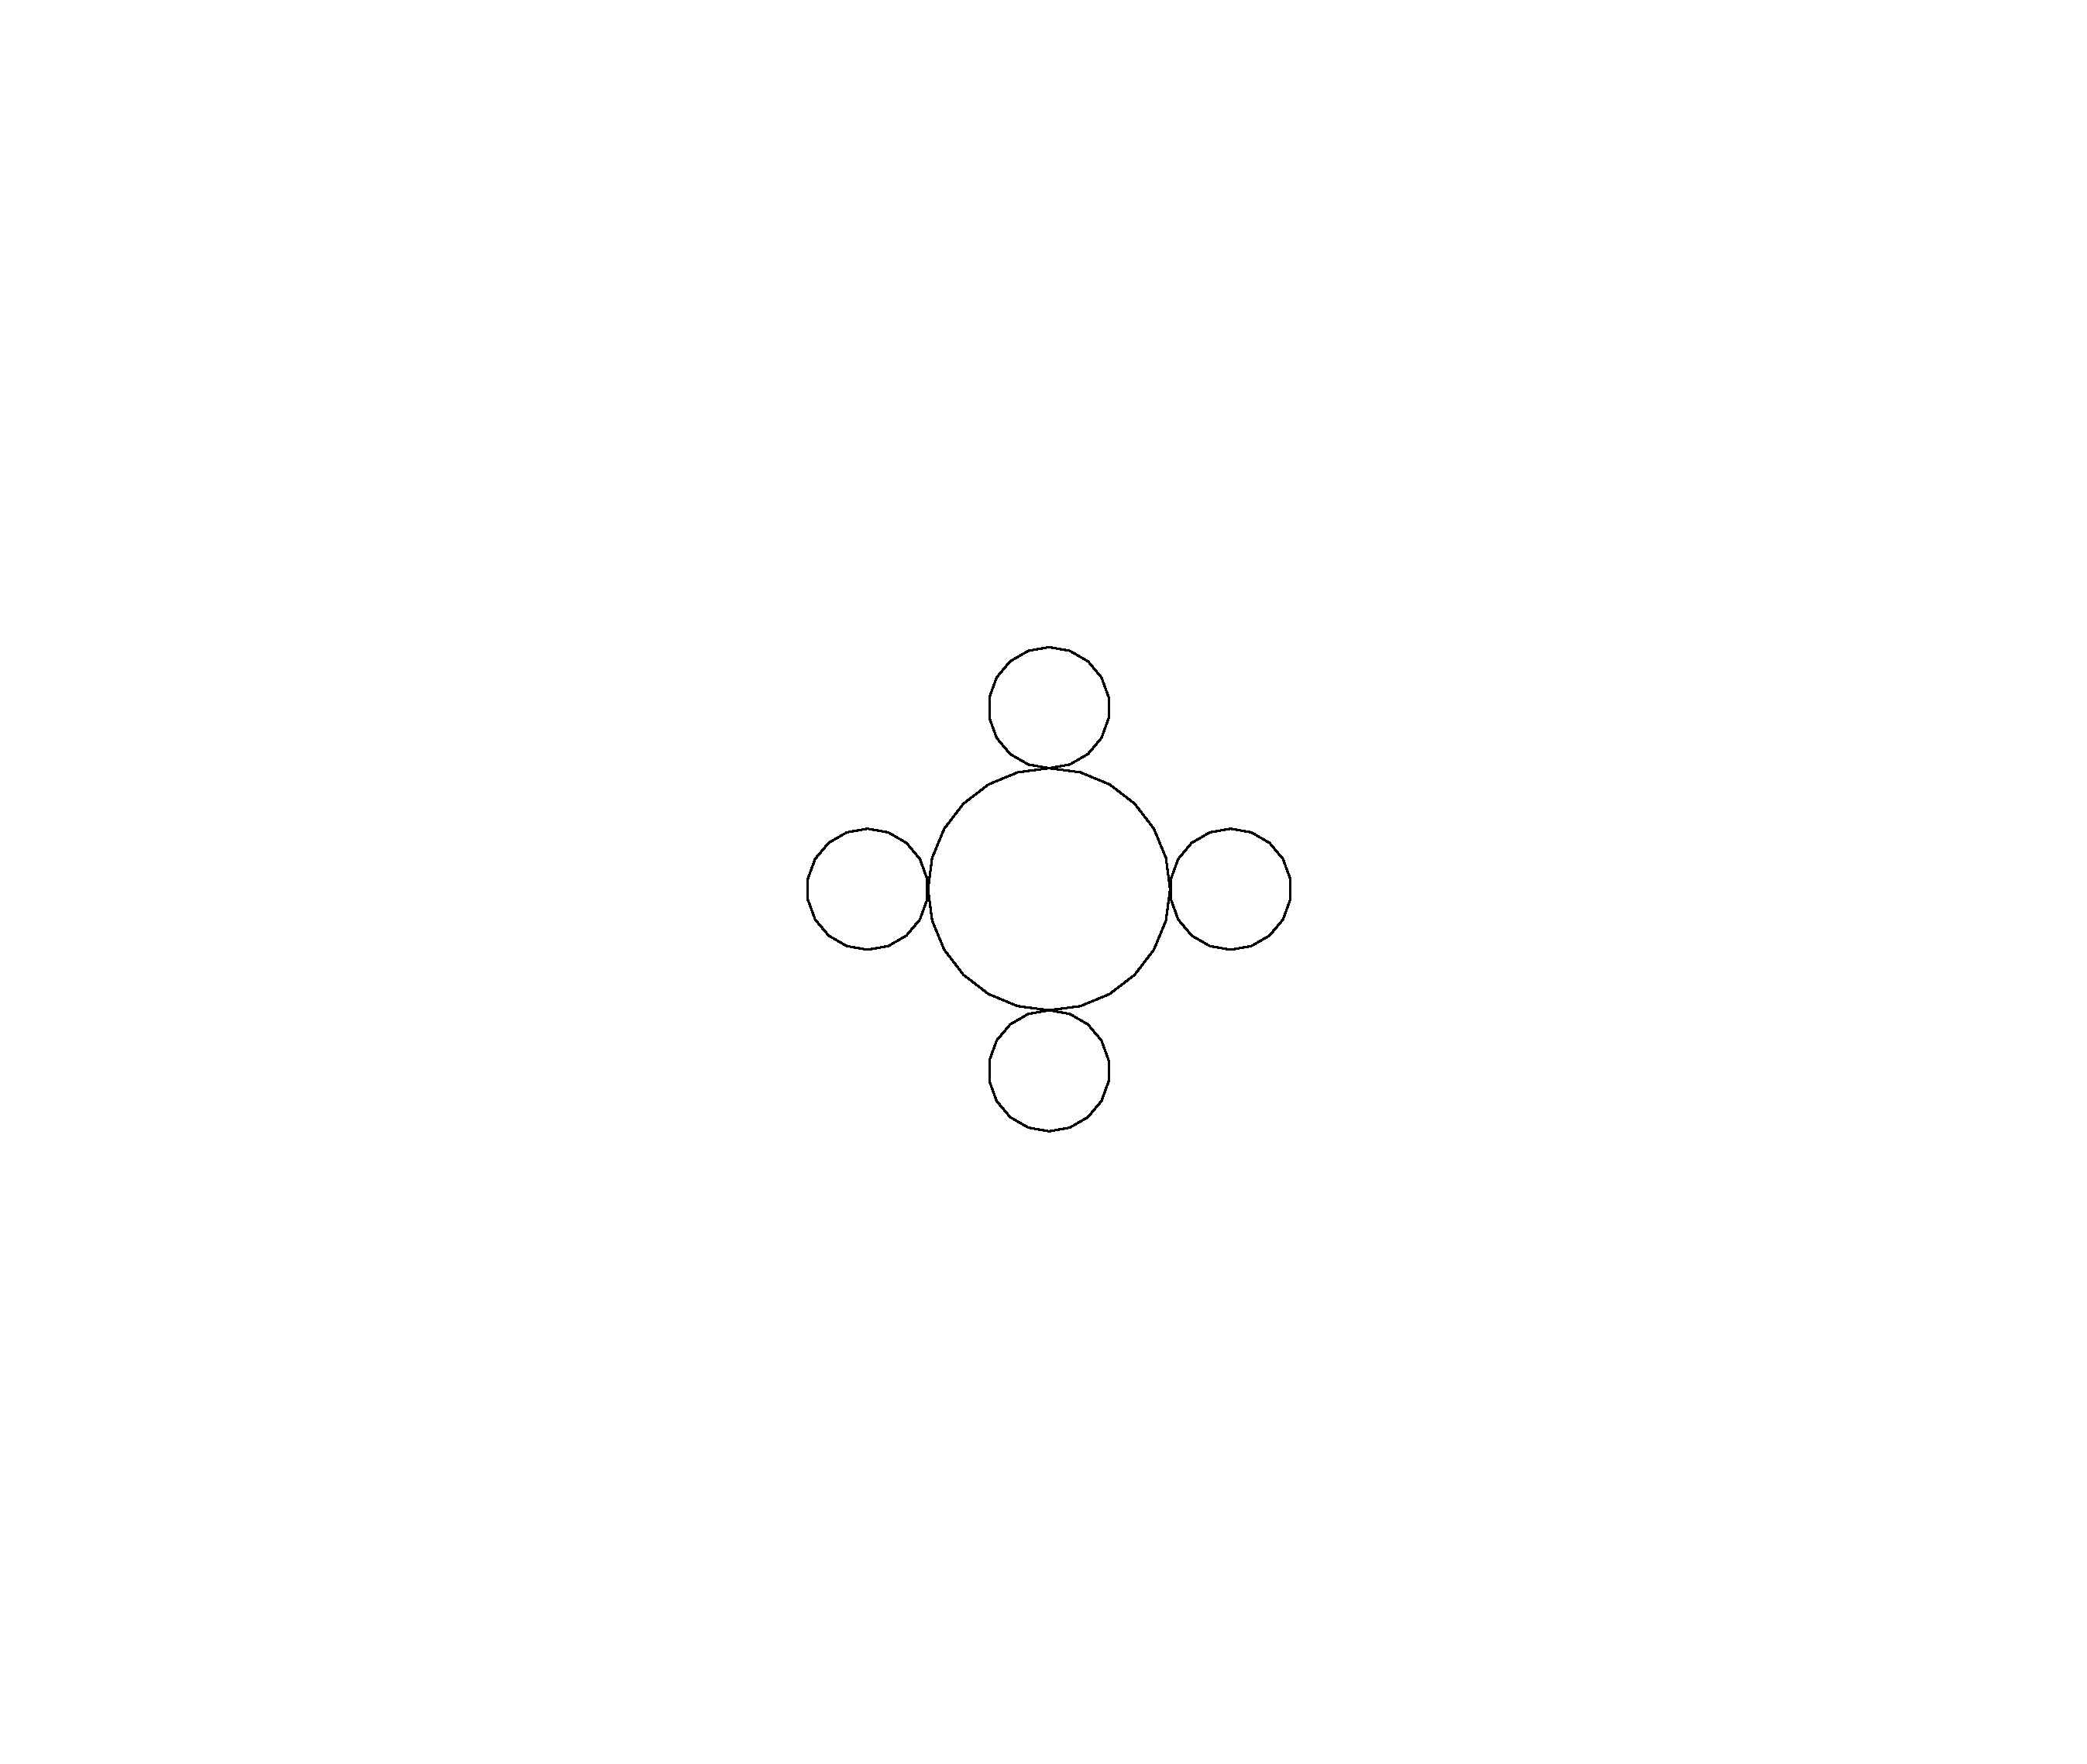
\includegraphics[trim=450 300 450 325,height=3.5cm]{2.eps}
}
\qquad
3 ~
\fbox{
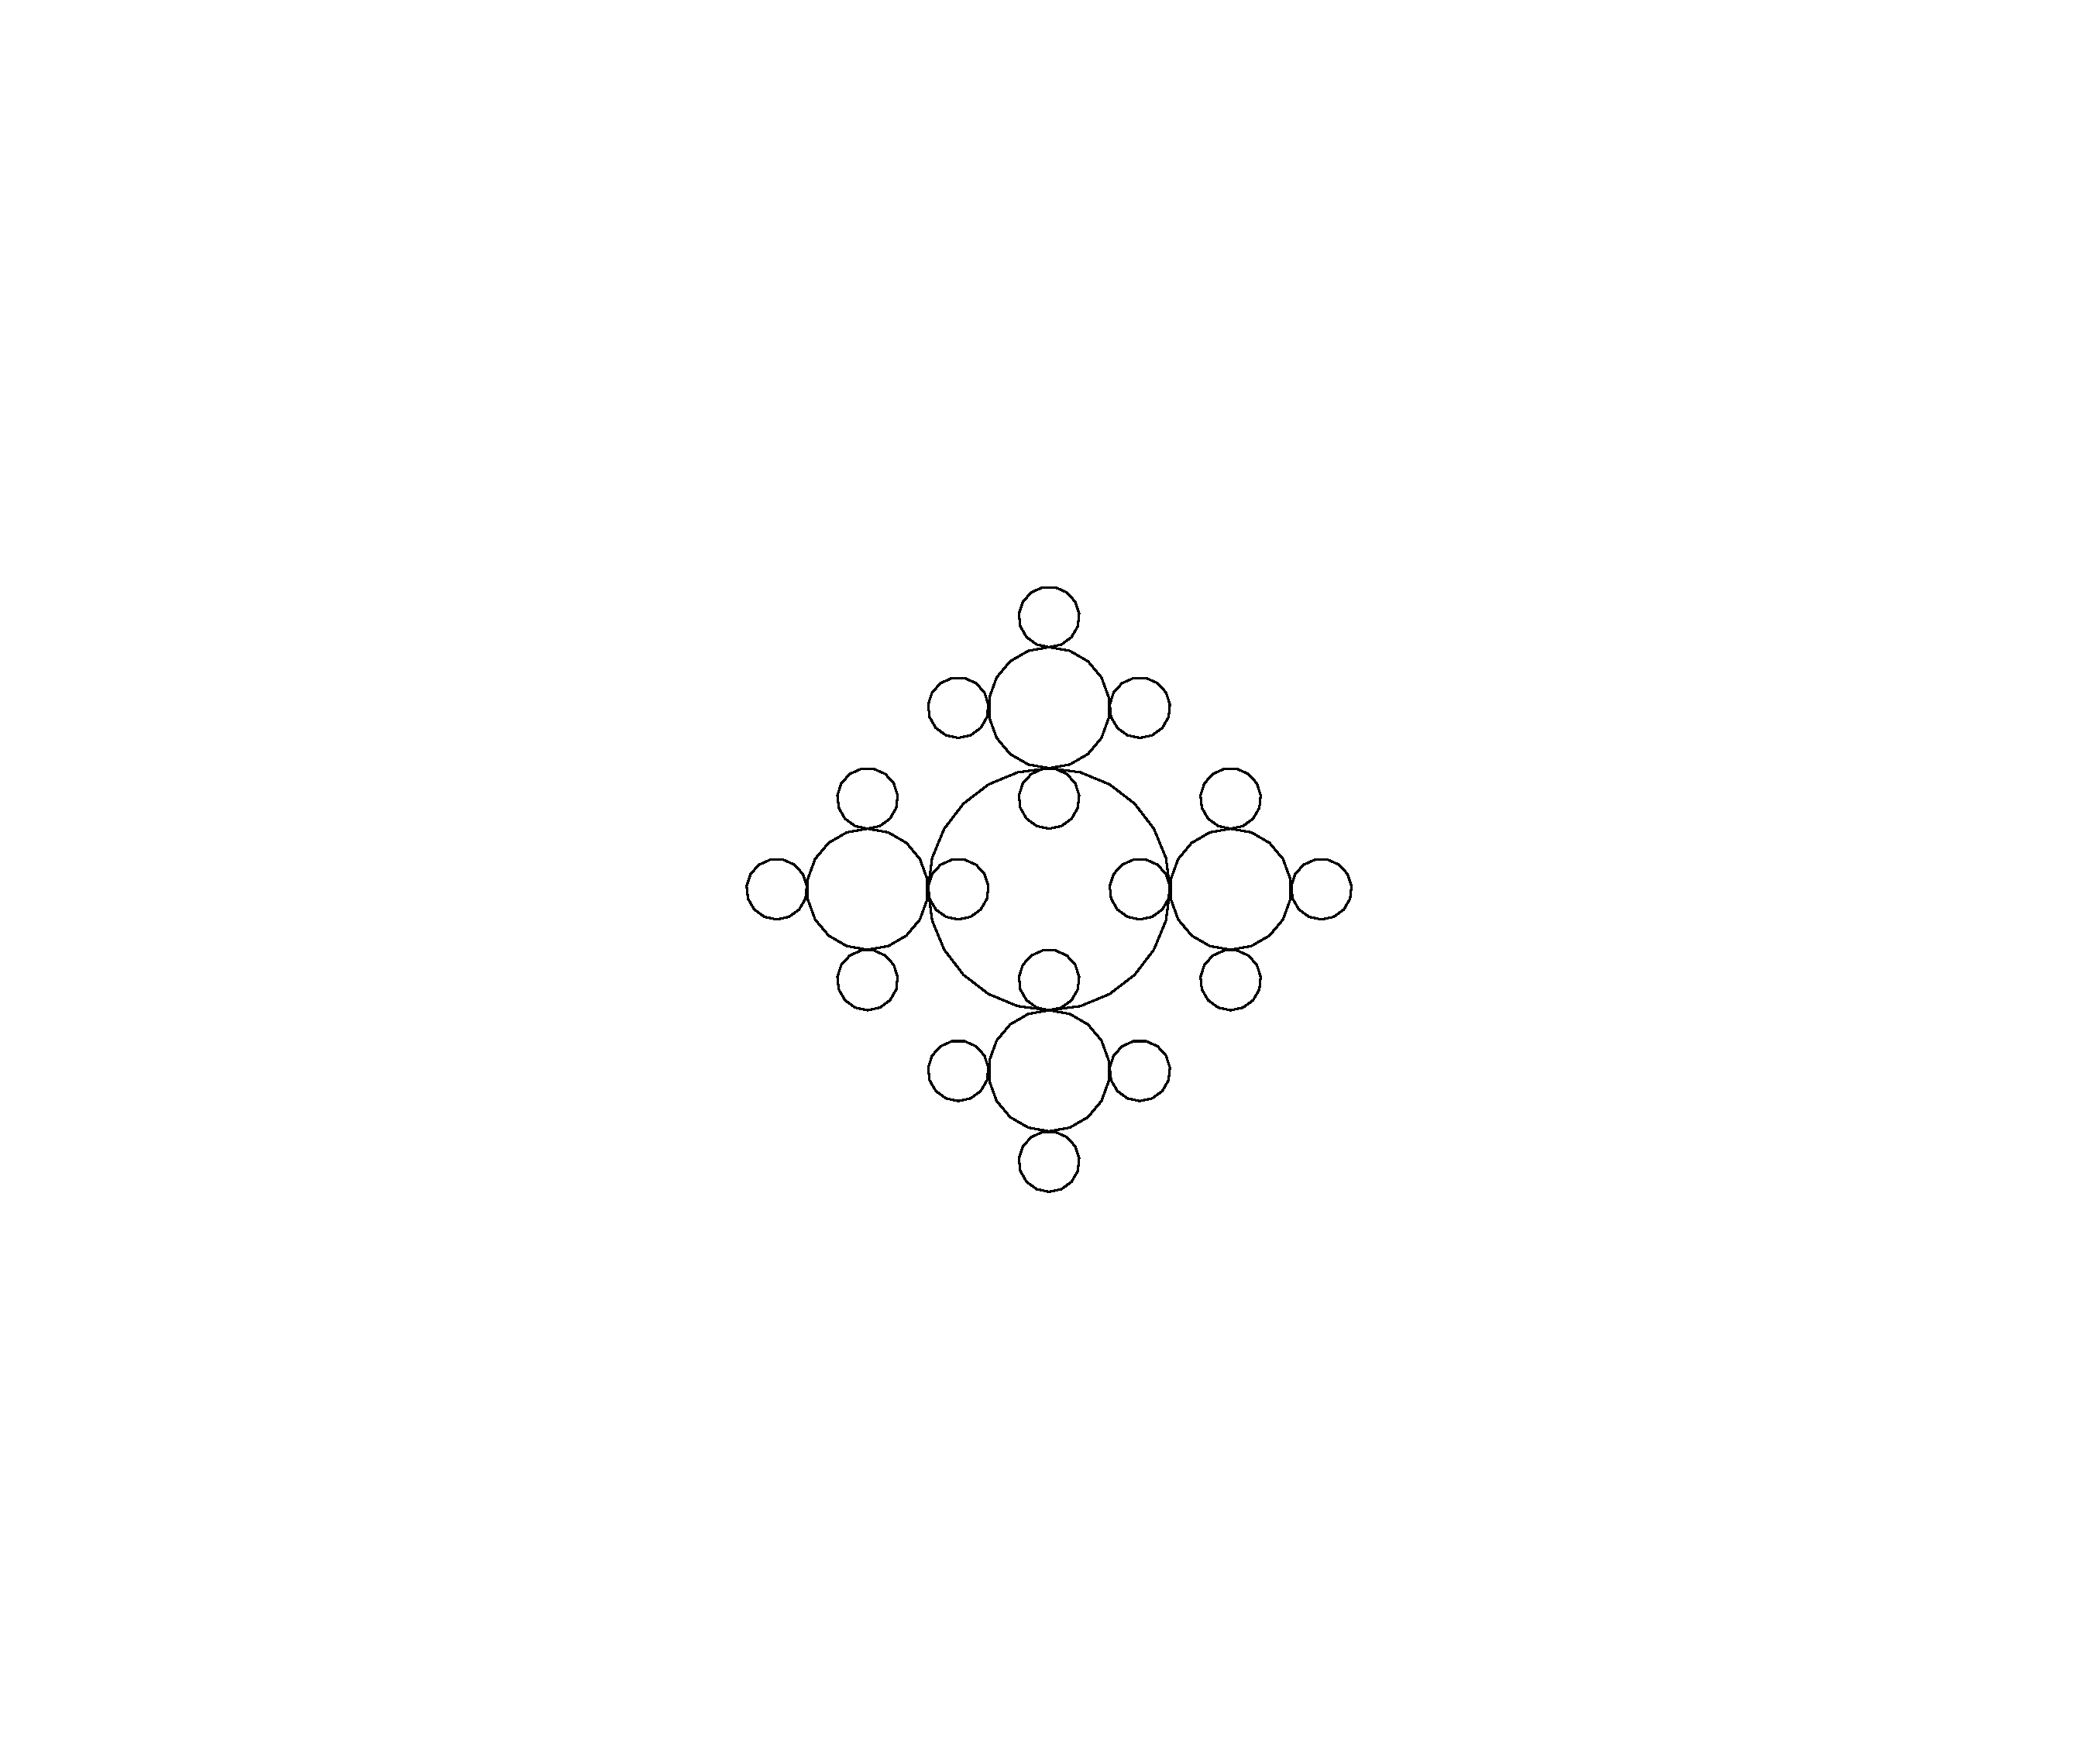
\includegraphics[trim=450 300 450 325,height=3.5cm]{3.eps}
}

\bigskip
\bigskip

4 ~
\fbox{
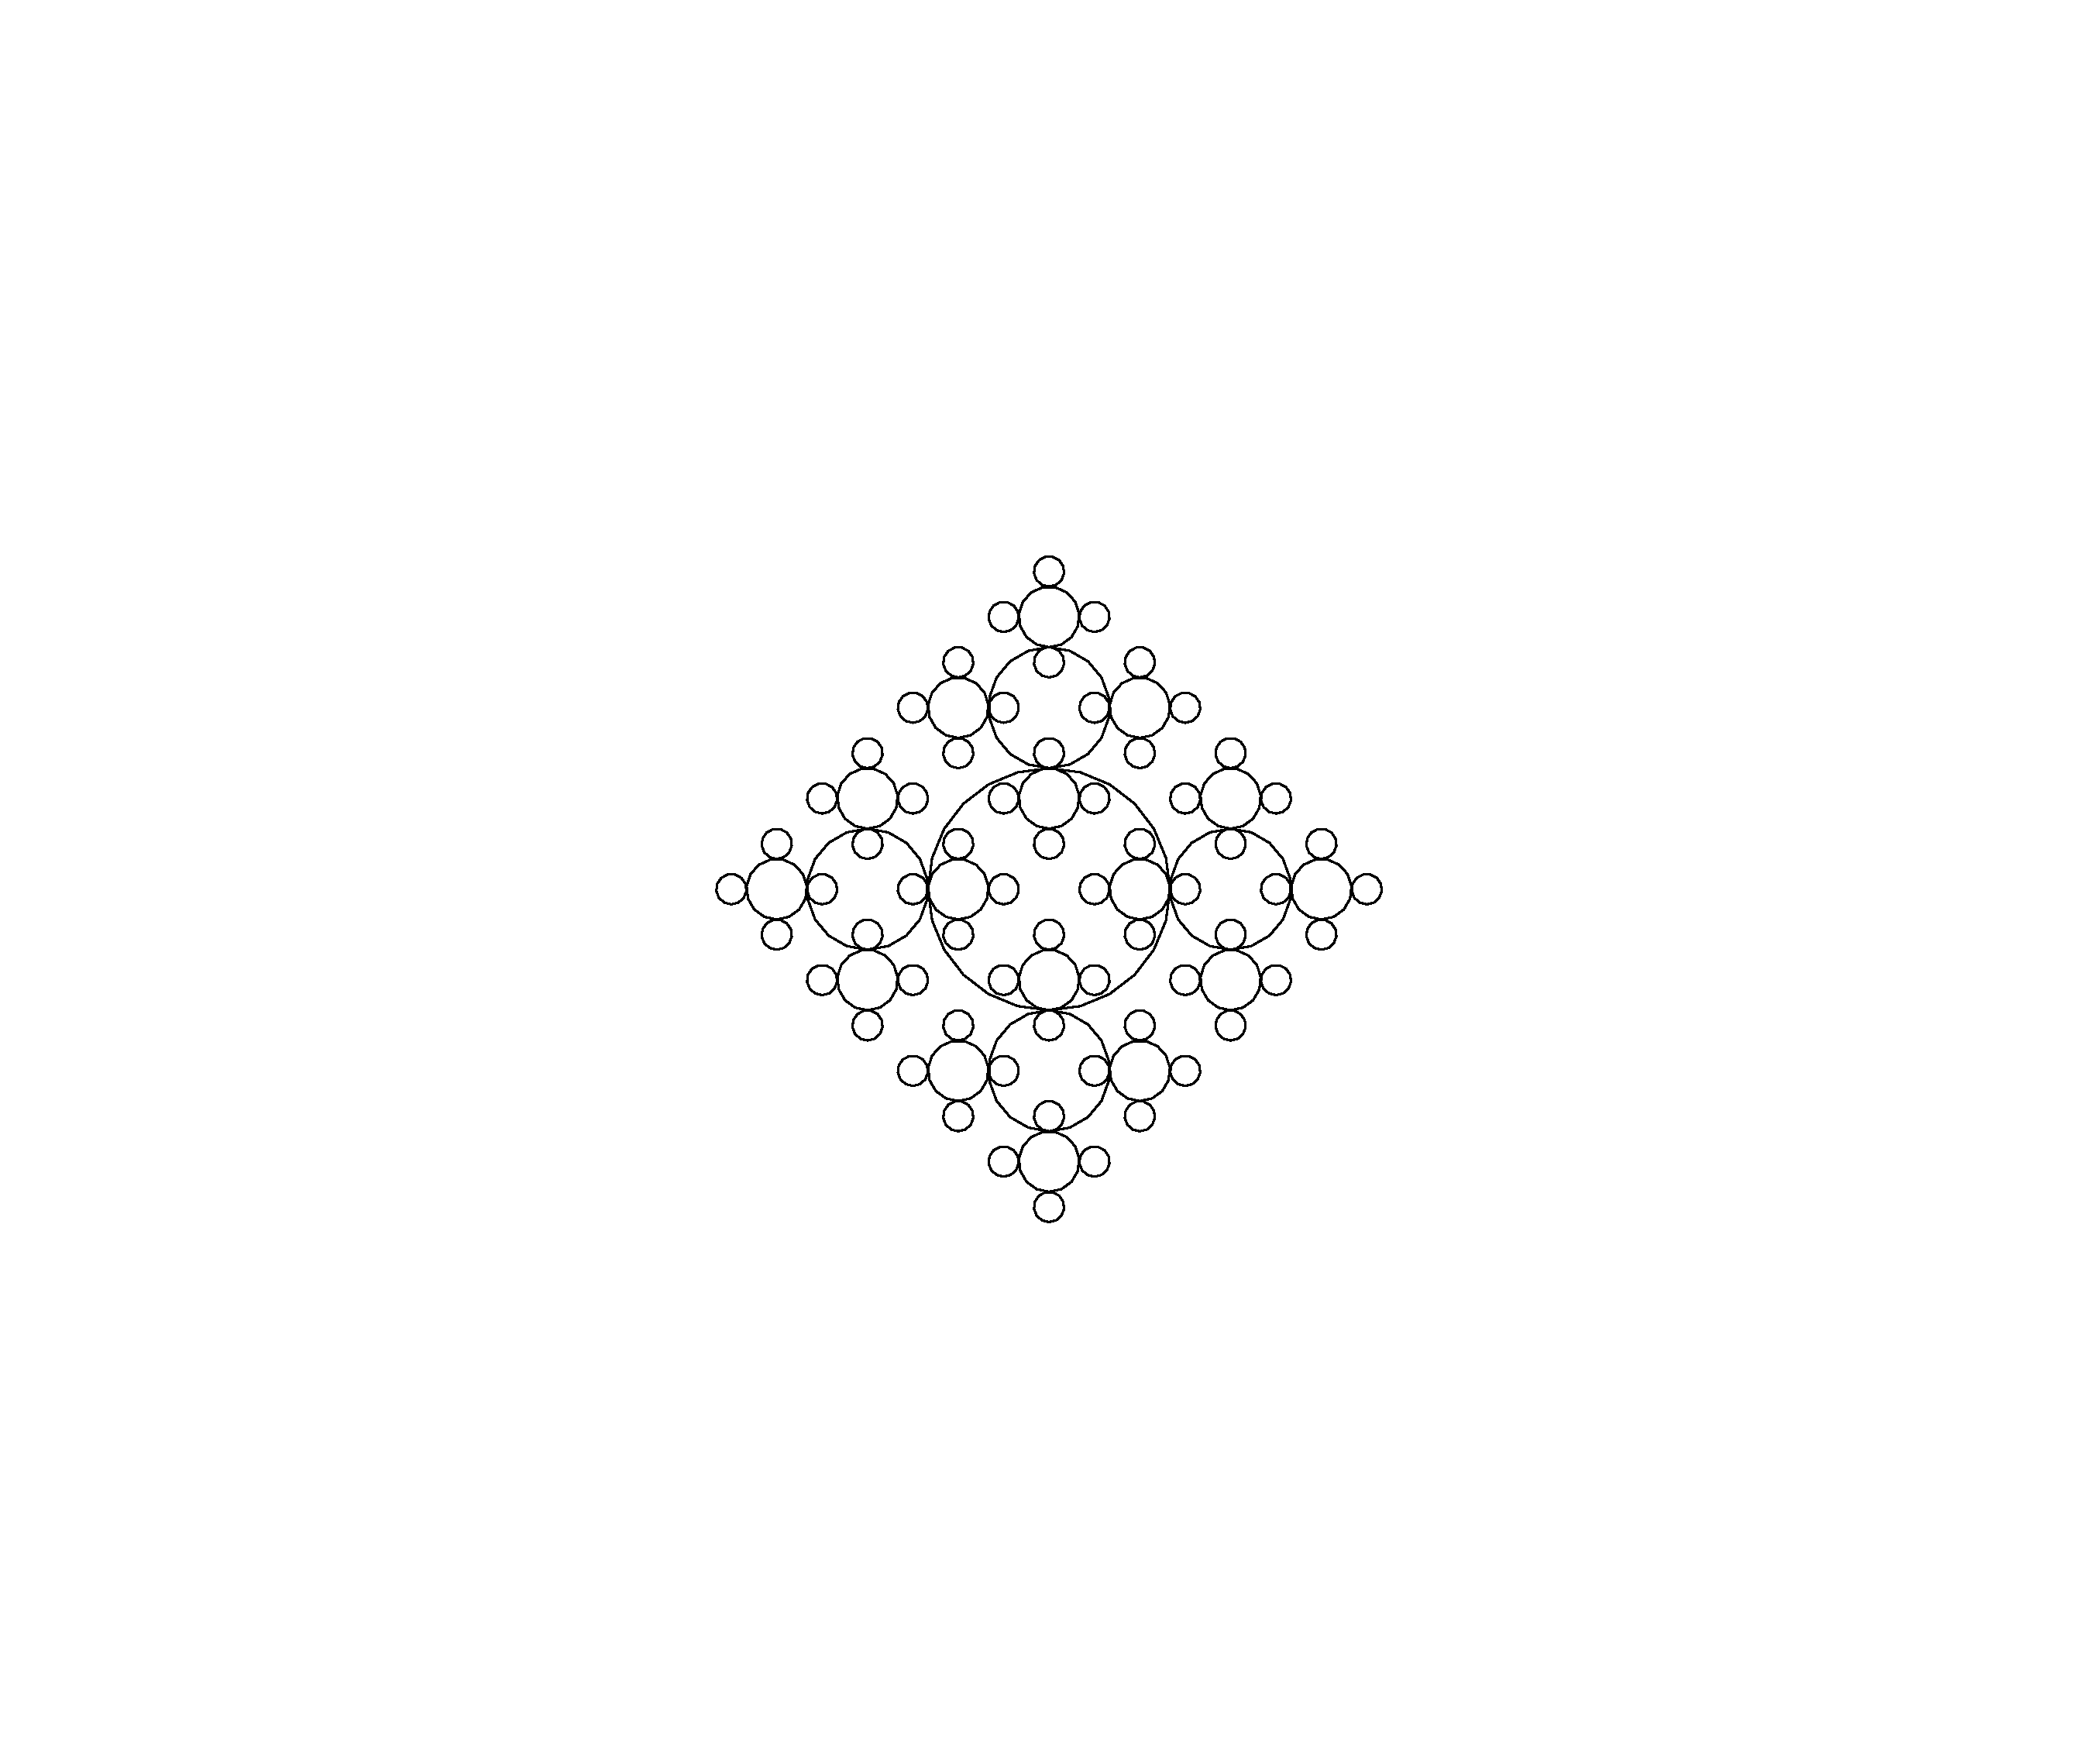
\includegraphics[trim=450 300 450 325,height=3.5cm]{4.eps}
}
\qquad
5 ~
\fbox{
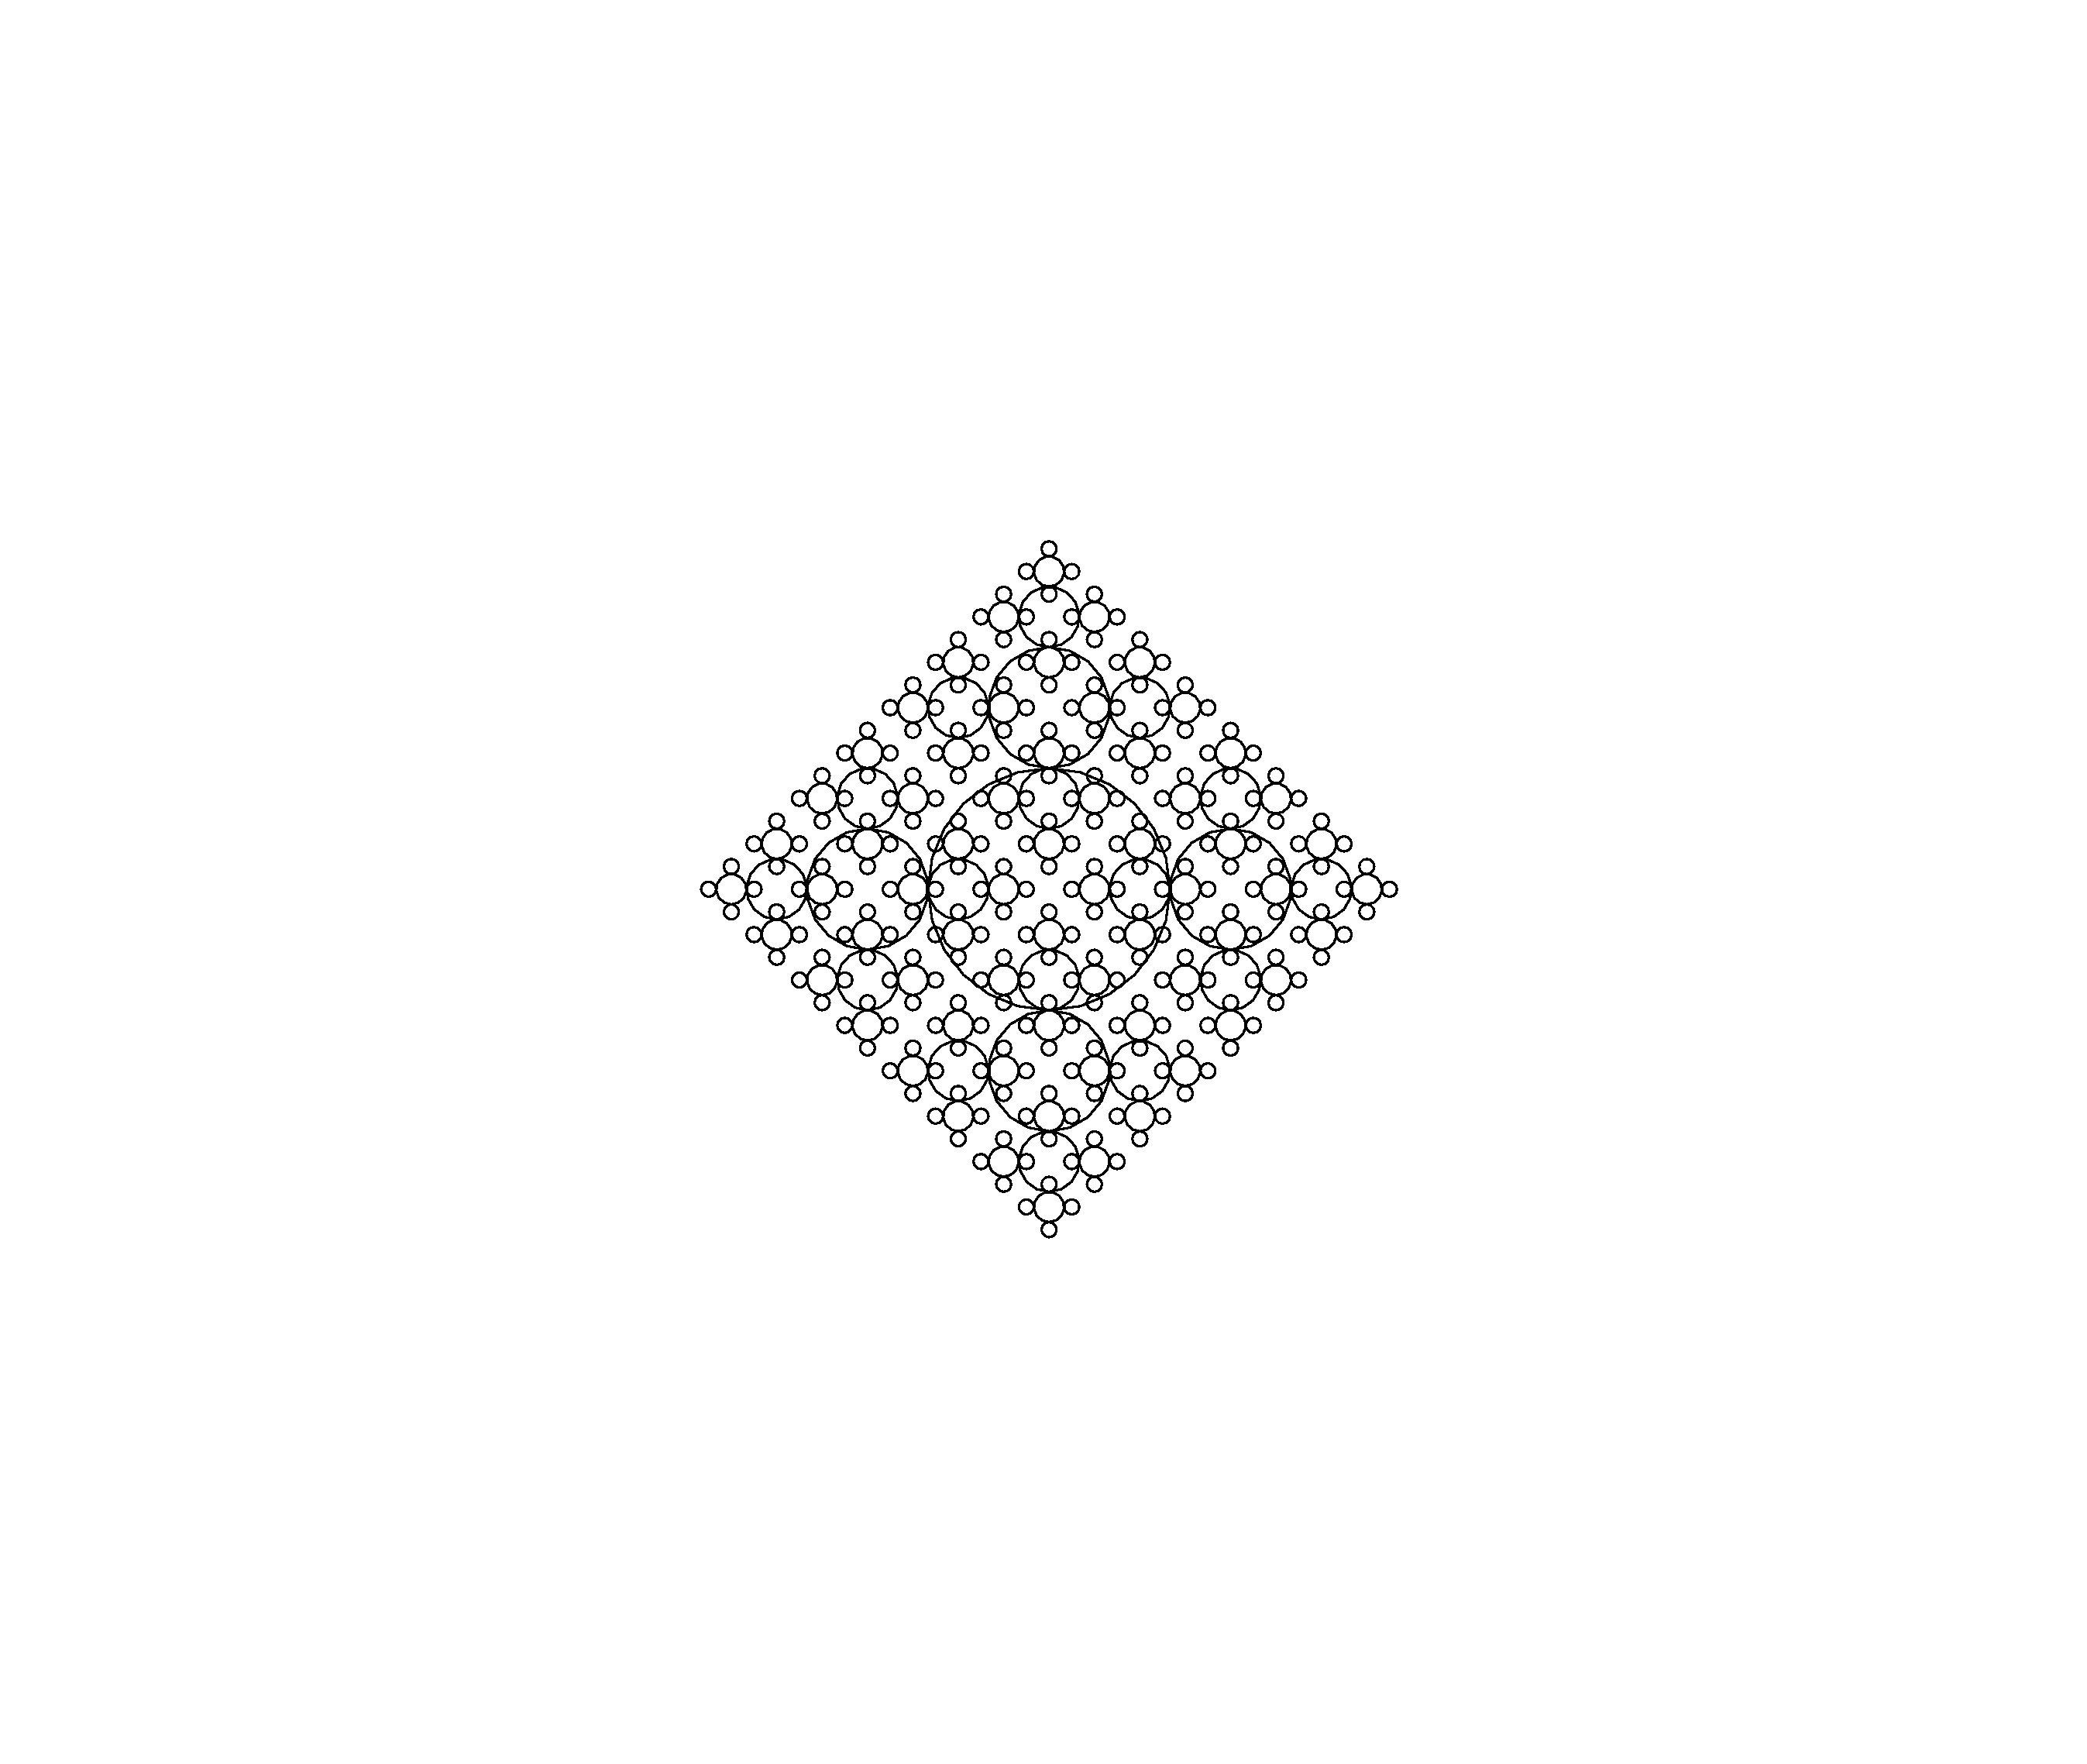
\includegraphics[trim=450 300 450 325,height=3.5cm]{5.eps}
}
\qquad
6 ~
\fbox{
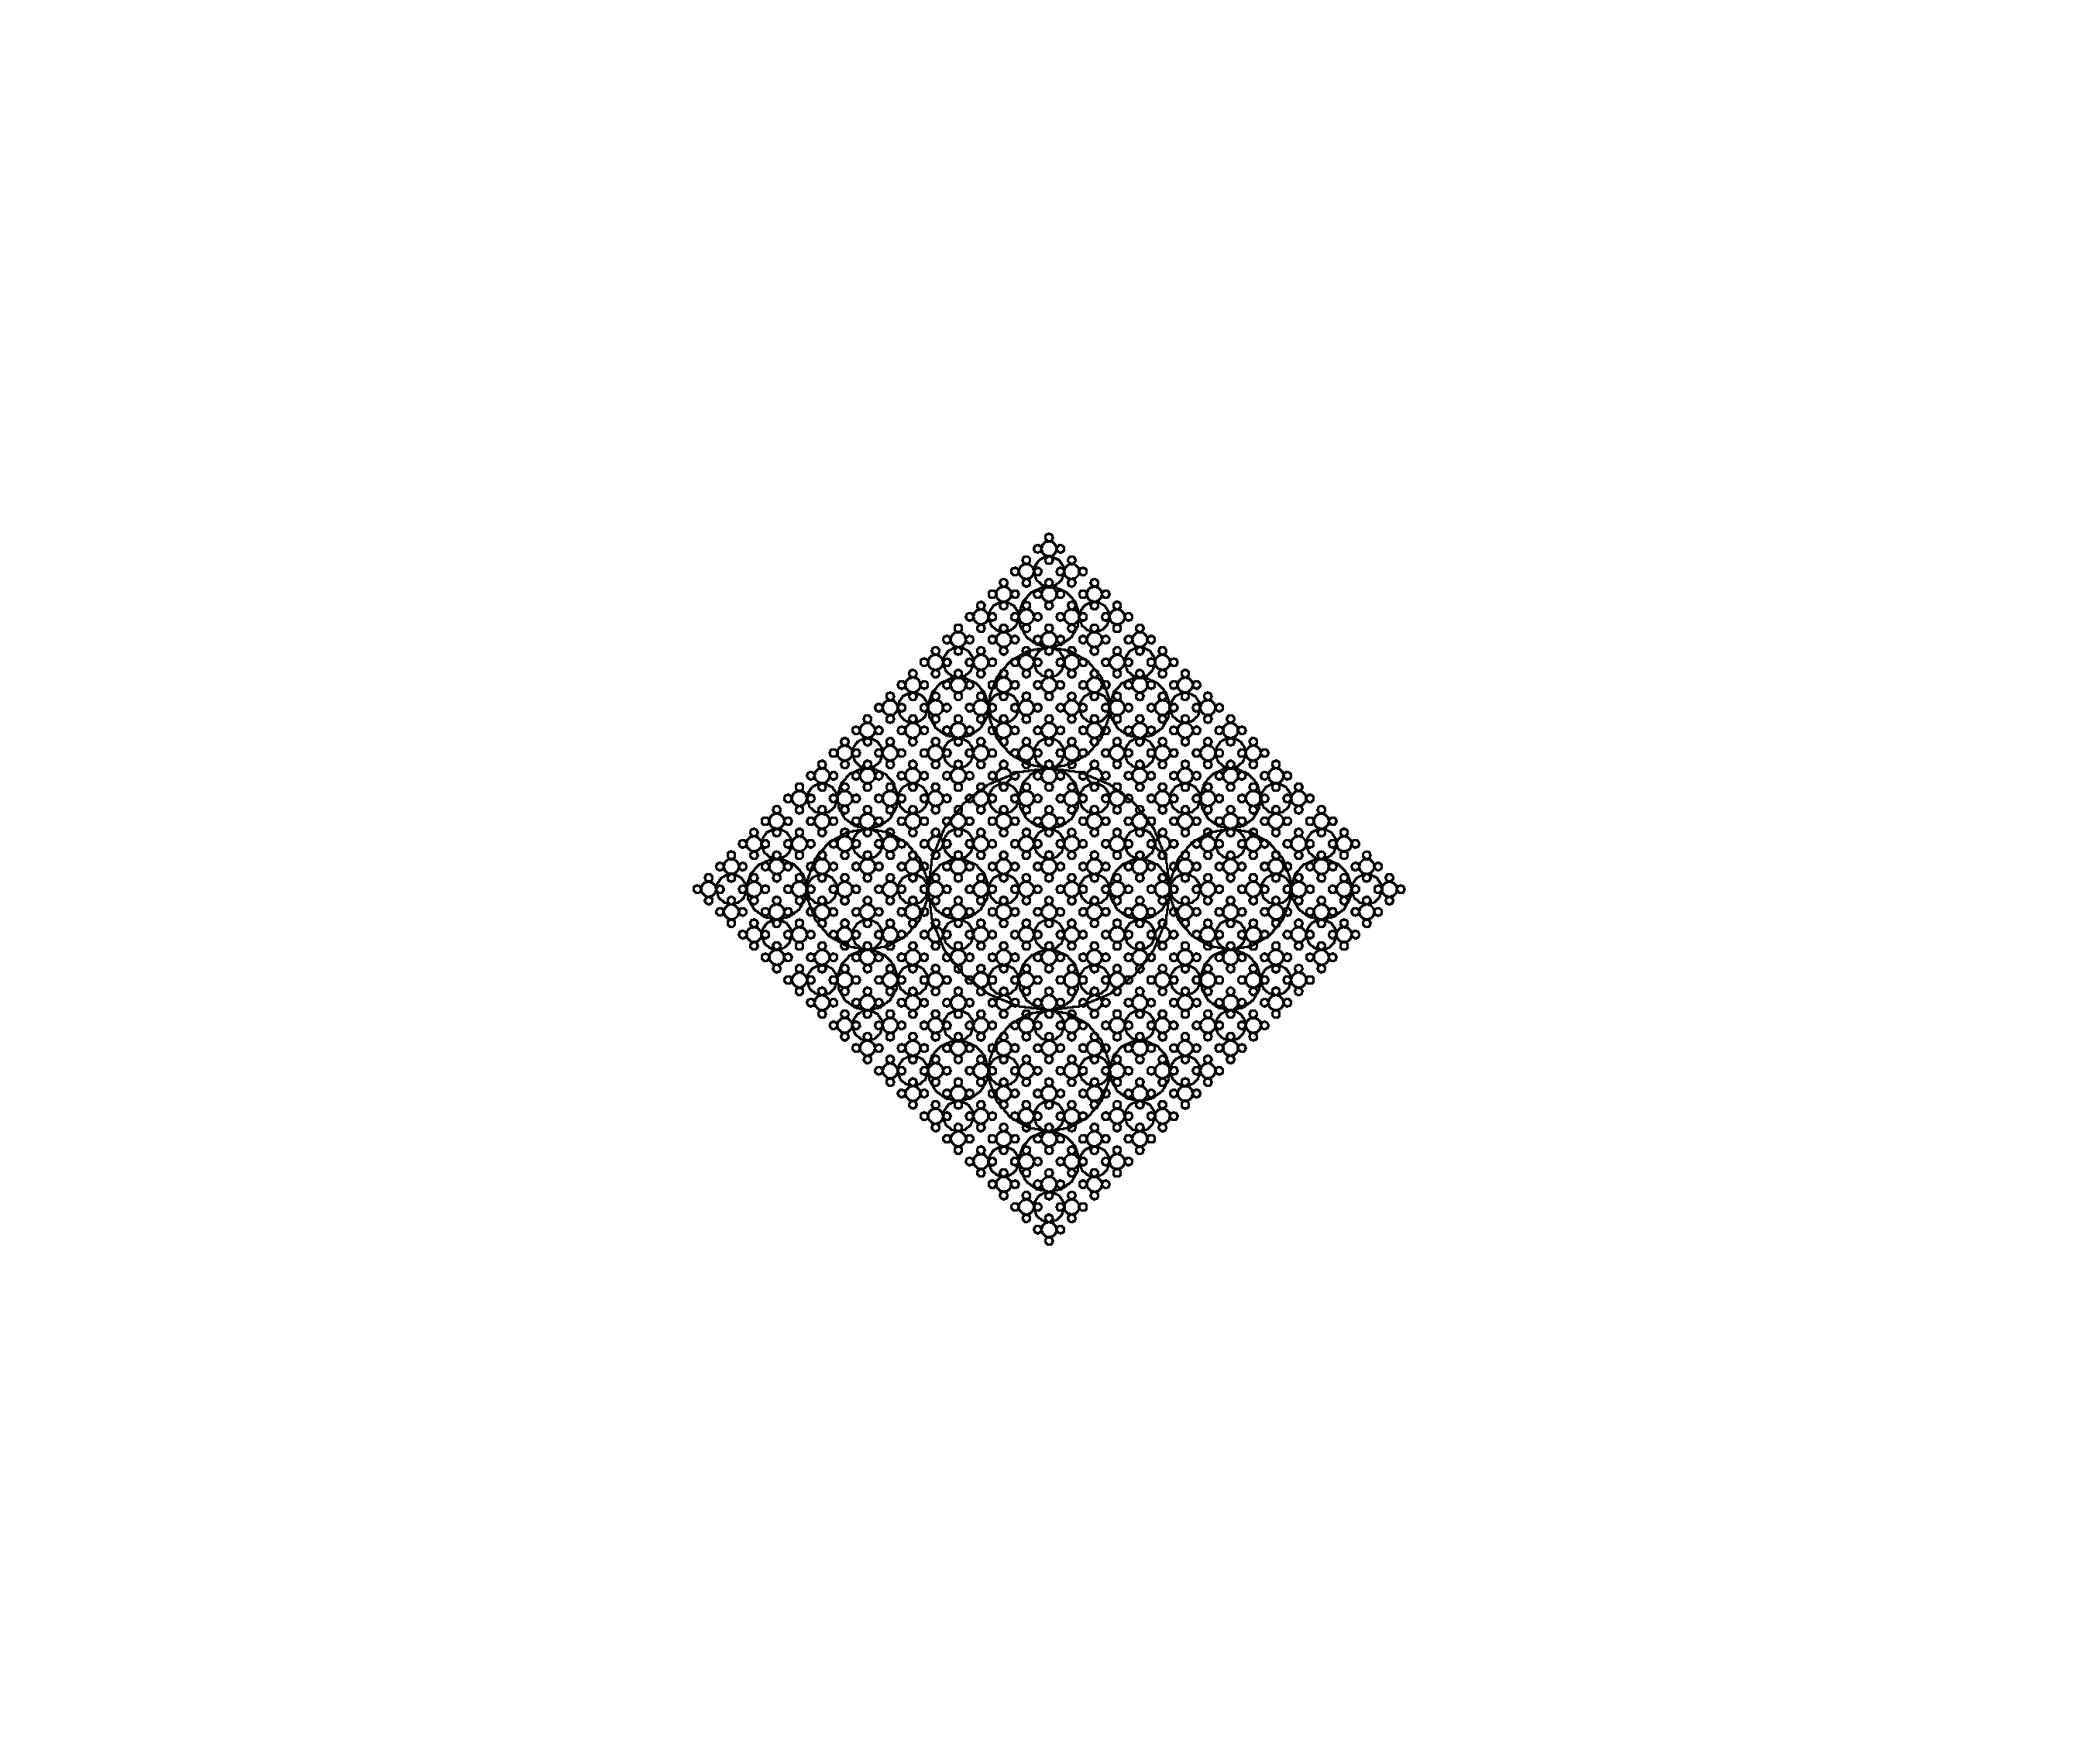
\includegraphics[trim=450 300 450 325,height=3.5cm]{6.eps}
}
\end{center}

\mysection{Entrada}

A l'entrada, es dónen dos valors: un natural $n$ amb el nombre de nivells del
fractal i un real positiu $d$ amb la seva mida.

\mysection{Sortida}

El programa ha de dibuixar el fractal d'$n$ nivells i
mida $d$ centrat a la finestra.

\bigskip

\begin{multicols}{2}\raggedcolumns
\mysection{Exemple d'entrada 1}

\begin{verbatim}
4
100
\end{verbatim}

\columnbreak

\mysection{Exemple de sortida 1}

\fbox{
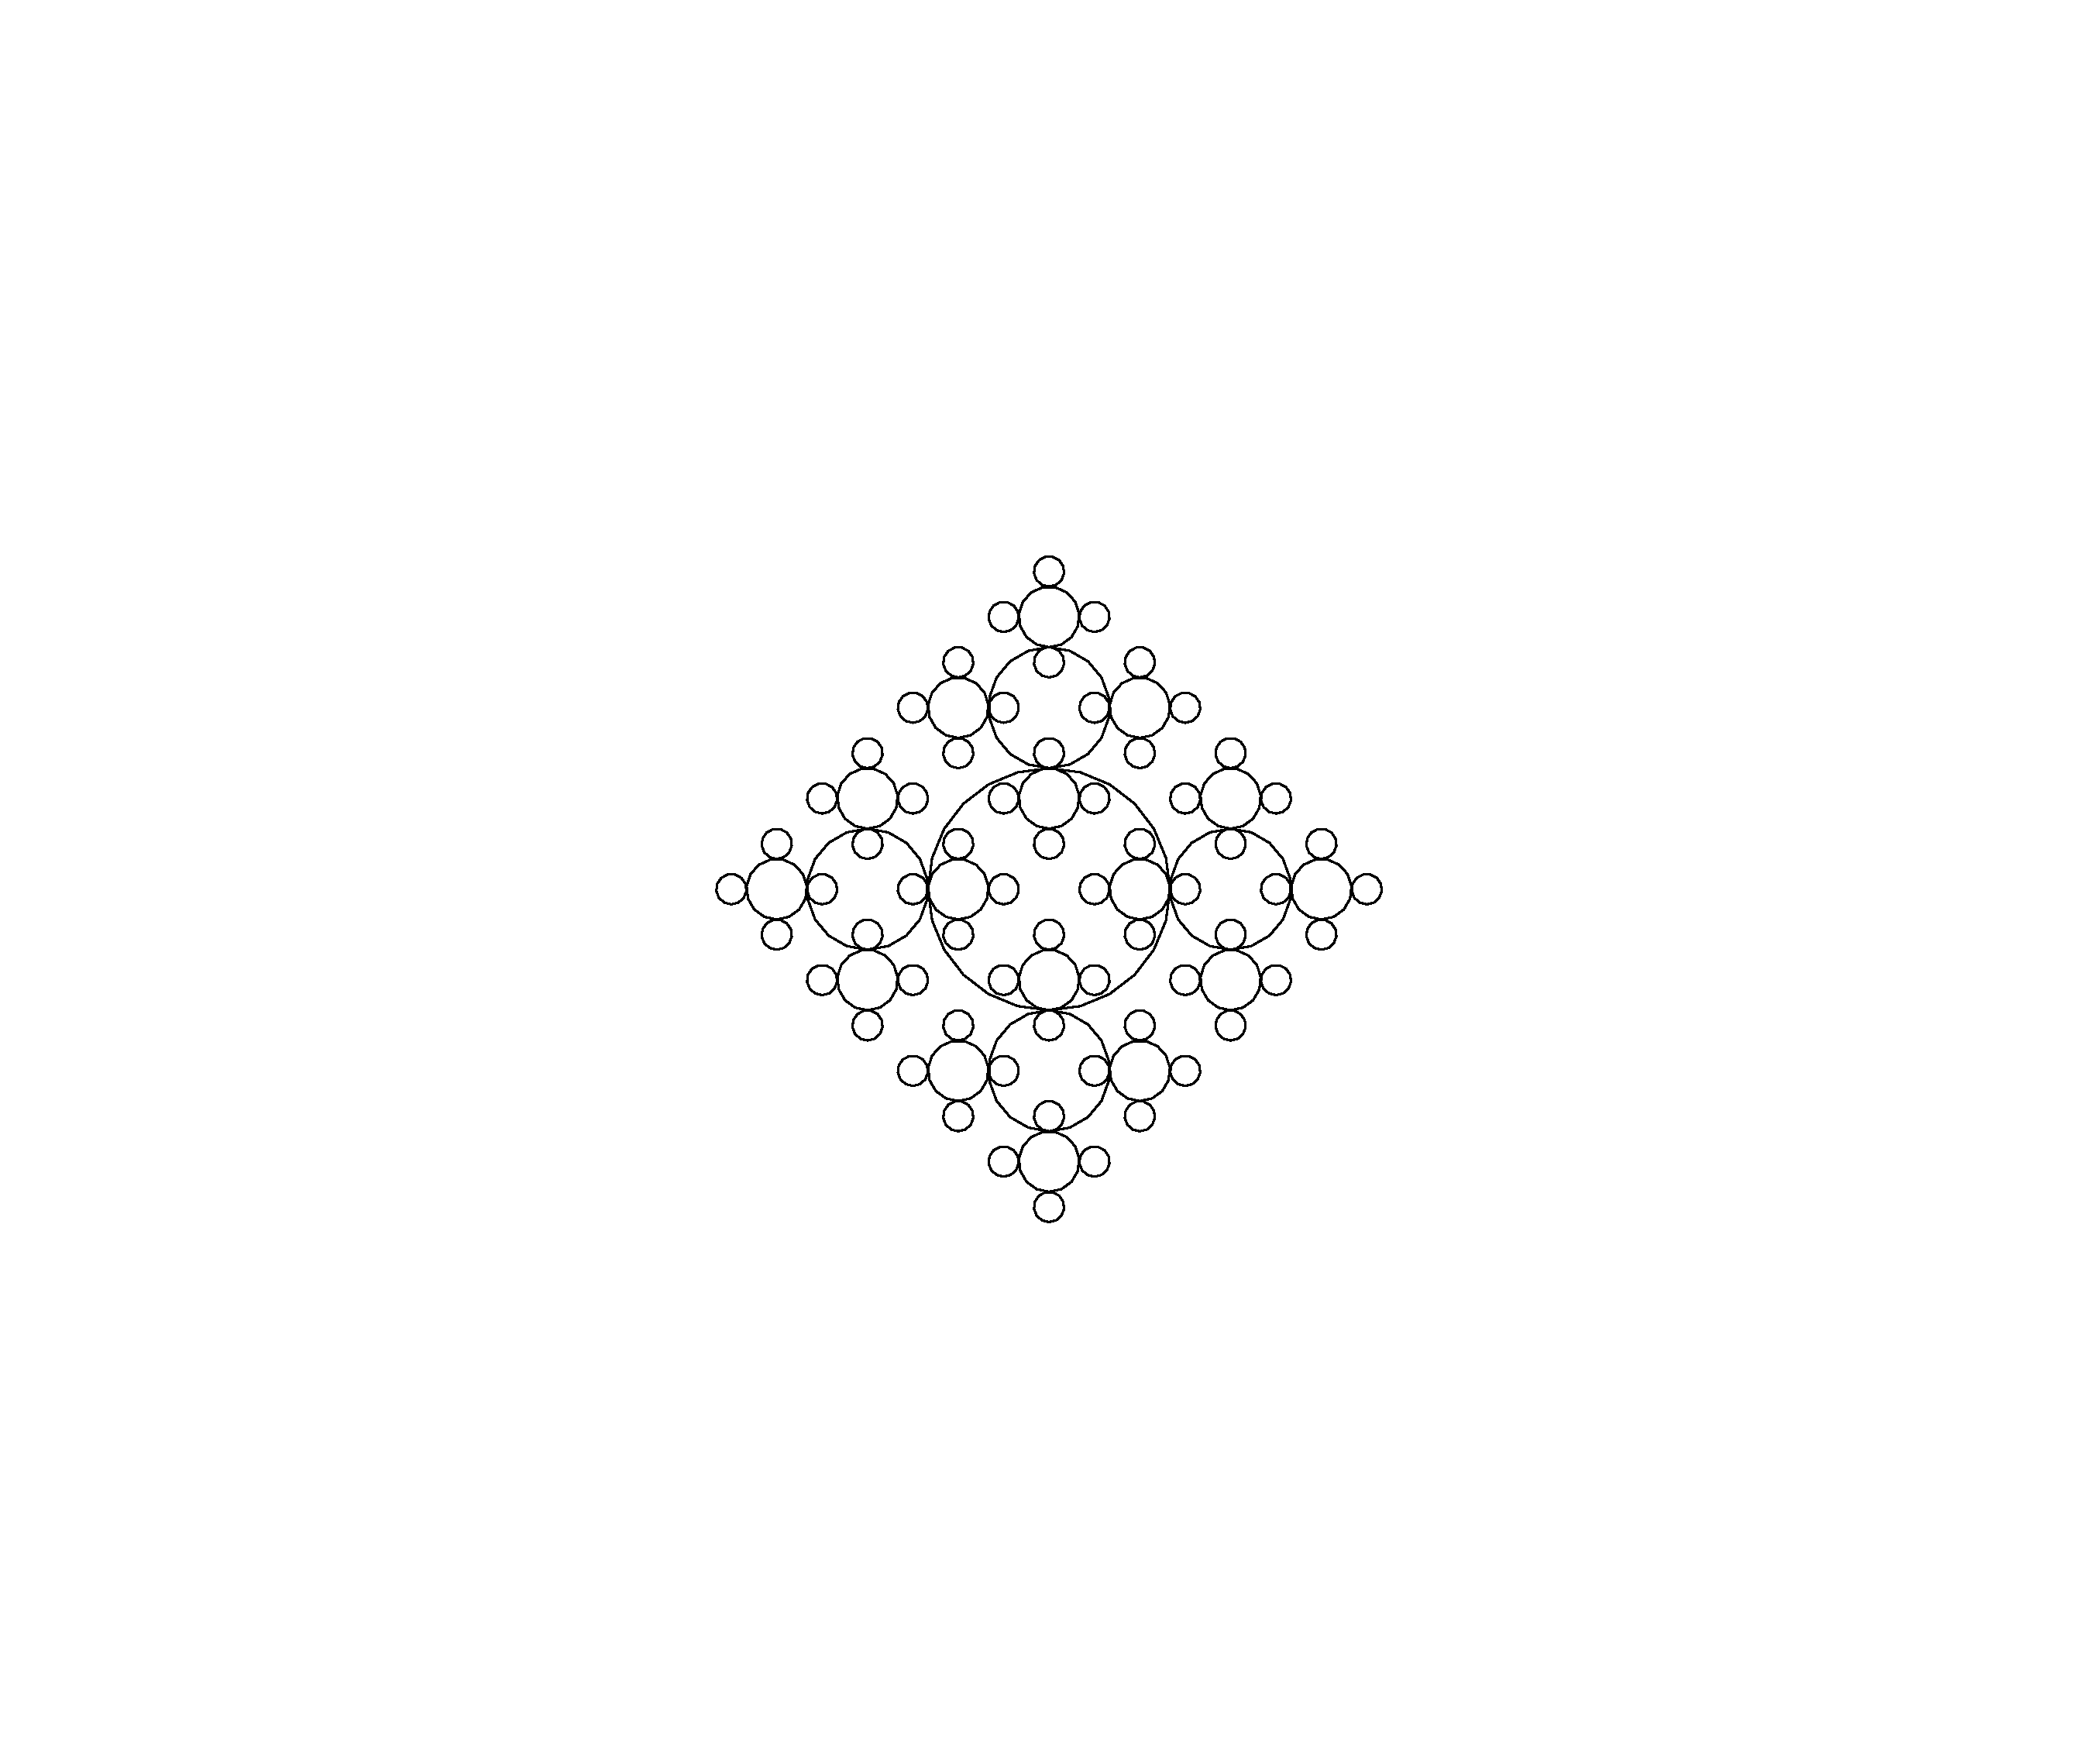
\includegraphics[trim=450 300 450 325,height=3.5cm]{sample1.eps}
}

\end{multicols}

\begin{multicols}{2}\raggedcolumns
\mysection{Exemple d'entrada 2}

\begin{verbatim}
2
50
\end{verbatim}


\columnbreak
\mysection{Exemple de sortida 2}

\fbox{

\includegraphics[trim=450 300 450 325,height=3.5cm]{sample2.eps}
}

\end{multicols}


\mysection{Recordatori}

Recordeu que Python ofereix un mòdul \texttt{turtle} que permet pintar images.
Les úniques operacions que us calen són
\texttt{turtle.goto(x, y)} que mou la tortuga a les coordenades (\texttt{x},\texttt{y}),
\texttt{turtle.circle(r)} que pinta un cercle de radi \texttt{r},
\texttt{turtle.down()} que activa el traçat i
\texttt{turtle.up()} que desactiva el traçat.

\bigskip

Per exemple, aquest programa pinta un cercle de mida \texttt{d} al mig de la finestra:

\begin{small}
\begin{verbatim}
import turtle
import yogi

d = yogi.read(float)
turtle.up()
turtle.goto(0, -d/2)
turtle.down()
turtle.circle(d)
\end{verbatim}
\end{small}

\mysection{Important}

Aquest problema no té jocs de proves al Jutge. Per tant, qualsevol solució serà
acceptada: semàfor verd! Això no vol dir que sigui bona ni dolenta, el vostre
professor ho corregirà.
